%! Author = timbe
%! Date = 05.02.2024

% Preamble
\documentclass[12pt]{article}

% Packages
\usepackage[left=3.0cm, right=1.5cm, top=2.0cm, bottom=2.0cm]{geometry}

\usepackage[utf8]{inputenc}
\usepackage[T2A]{fontenc}
\usepackage[russian]{babel}
\usepackage{amsmath, amsfonts, amssymb}
\usepackage{graphicx}
\usepackage{wrapfig}
\usepackage{fancyhdr}
\usepackage[shortlabels]{enumitem}
\usepackage{svg}
\usepackage{amstex}
\usepackage{colortbl}
\usepackage{bm}

\renewcommand{\vec}{\textbf}
\newcommand{\cross}{\times}

\pagestyle{fancy}
\fancyhead[L]{Работа №4.5.2}
\fancyhead[R]{Белинский Т.Д.\quad Б05-206}

% Document
\begin{document}
    \section*{4.5.2. ИНТЕРФЕРЕНЦИЯ ЛАЗЕРНОГО ИЗЛУЧЕНИЯ}
    \ \par
    \textbf{Цель работы:} исследование видности интерференционной картины излучения
    гелий-неонового лазера и определение длины когерентности излучения. \par
    \textbf{Оборудование:} He-Ne-лазер, интерферометр Майкельсона с подвижным зеркалом,
    фотодиод с усилителем, осциллограф, поляроид, линейка.

    \subsection*{Теоретическая часть}
    \ \par
    Лазер - источник квазимонохроматического и узконаправленного высококогерентного потока излучения,
    работающий за счет эффекта вынужденного излучения.
    Главные элементы лазера - оптический резонатор и расположенная в нем активная среда.
    Время когерентности - время, на которое можно задержать пучок относительного другого,
    чтобы еще сохранялась способность к интерференции между ними.
    При геометрических задержках кратных удвоенной длине резонатора,
    интерференция пучков должна восстанавливаться.

    Важный параметр интерференционной картины --- ее видность:

    \begin{equation}
        \label{eq:eq1}
        \mathcal{\mathcal{V}} = \dfrac{I_{max} - I_{min}}{I_{max} + I_{min}}.
    \end{equation}

    Представлять видность удобно как произведение функций различных параметров установки/системы:

    \begin{equation}
        \label{eq:eq2}
        \mathcal{V} = \mathcal{V}_1 \mathcal{V}_2 \mathcal{V}_3
    \end{equation}

    $\mathcal{V}_1$ отвечает за отношение интенсивностей интерферирующих волн:

    \begin{equation}
        \label{eq:eq3}
        \mathcal{V}_1 = \dfrac{2\sqrt{\delta}}{1 + \delta}, \quad \delta = \dfrac{B_m^2}{A_m^2},
    \end{equation}
    где $ A_m, B_m $ --- амплитуды волн.

    $\mathcal{V}_2$ учитывает влияние разности хода и спектрального состава волн:

    \begin{wrapfigure}[8]{r}{0.37\linewidth}
        \label{fig:fig1}
        \centering
        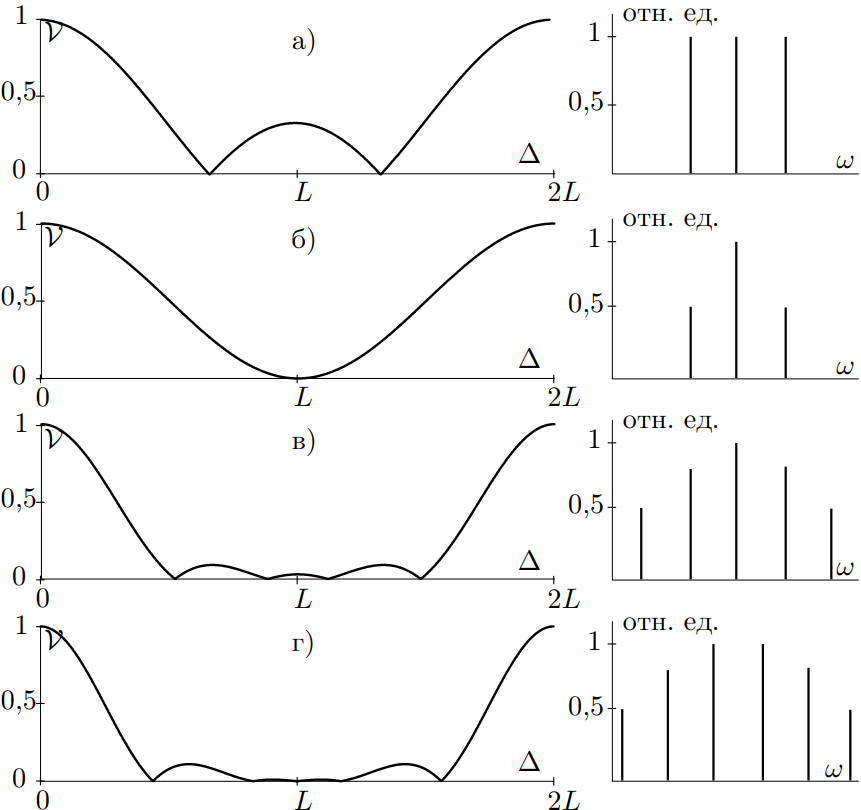
\includegraphics[width=\linewidth]{pic/v2}
        \caption{Зависимость видности от задержки для разного количества мод}
    \end{wrapfigure}

    \begin{equation}
        \label{eq:eq4}
        \mathcal{V}_2=\left|\frac{1}{n}\frac{\sin\frac{\pi l}{2L}n}{\sin\frac{\pi l}{2L}}\right|,
    \end{equation}
    где $l$ --- разность хода, $L$ -- расстояние между зеркалами.

    $\mathcal{V}_3$ учитывает влияние различности поляризации волн.
    Если волны поляризованы линейно, то выражение для видности будет иметь следующий вид
    \begin{equation}
        \label{eq:eq5}
        \mathcal{V}_3 = |\cos \alpha|,
    \end{equation}
    если же волны имеют линейную поляризацию,
    но направление поляризации хаотически меняется от 0 до $\pi$, то можно получить:

    \begin{equation}
        \label{}
        \mathcal{V}_3 = \left|\cos^2{\alpha}\right|,
    \end{equation}
    где $\alpha$ -- угол между плоскостями поляризации

    \subsection*{Экспериментальная установка}
    \ \par
    \begin{wrapfigure}[21]{l}{0.7\linewidth}
        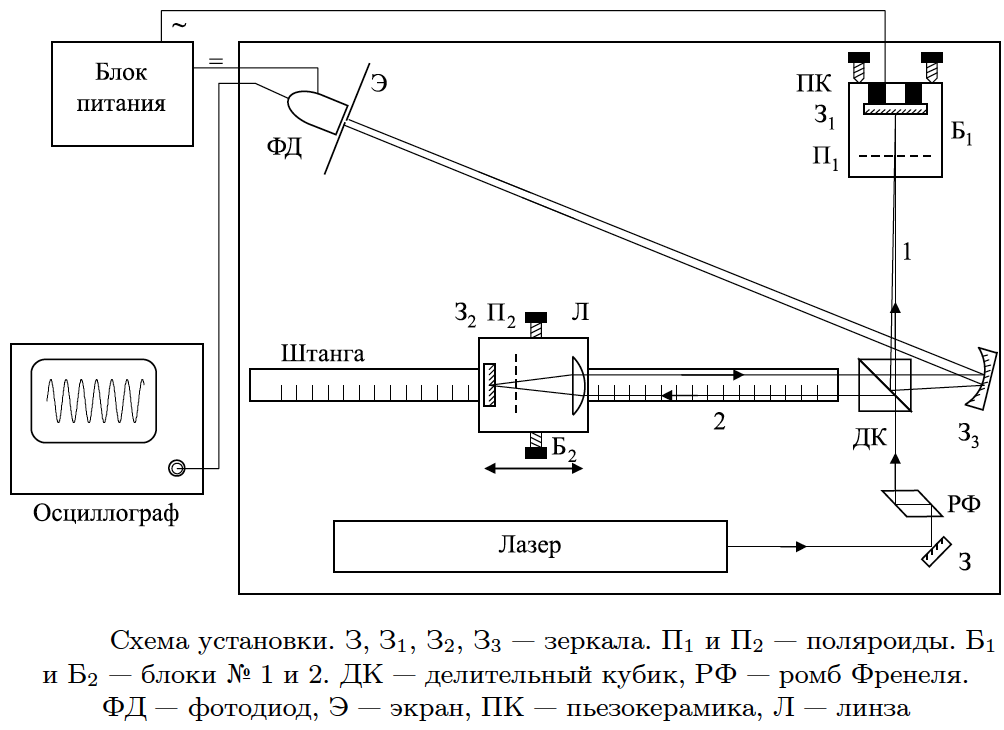
\includegraphics[width=\linewidth]{pic/setup}
        \caption{Экспериментальная установка}
        \label{fig:fig2}
    \end{wrapfigure}

    Для получения интерференционной картины используется интерферометр Майкельсона,
    смонтированный на вертикально стоящей массивной металлической плите.
    Схема установки приведена на рисунке\ \ref{fig:fig2}.

    Источником света служит гелий-неоновый лазер (средняя длина
    волны $ \lambda_0 = 632,8 $ нм).
    Пучок лазерного излучения отражается от зеркала З и проходит призму полного внутреннего отражения
    РФ (ромб Френеля), которая превращает линейную поляризацию излучения в круговую.
    Если в установке используется лазер, излучающий неполяризованный свет, то ромб Френеля не нужен,
    но он и не мешает выполнению работы.
    Далее лазерное излучение делится диагональной плоскостью делительного кубика ДК на два пучка.

    Пучок 1 проходит поляроид $ \text{П}_1 $, отражается под небольшим углом от зеркала $ \text{З}_1 $,
    снова проходит поляроид $ \text{П}_1 $, и частично отражаясь от диагональной плоскости
    делительного кубика, выходит из интерферометра, попадает на зеркало $ \text{З}_3 $
    и далее на фотодиод ФД.
    Зеркало $ \text{З}_1 $ наклеено на пьезокерамику ПК,
    которая может осуществлять малые колебания зеркала вдоль направления распространения падающего пучка.
    Поляроид и зеркало с пьезокерамикой собраны в единый блок $ \text{Б}_1 $,
    который крепится к вертикально стоящей плите.
    В блоке $ \text{Б}_1 $ имеются юстировочные винты, которые позволяют регулировать
    угол наклона зеркала $ \text{З}_1 $.
    В установке предусмотрена возможность вращения поляроида $ \text{П}_1 $.
    Угол поворота отсчитывается по шкале, нанесённой на оправу поляроида.
    Пучок 2 проходит линзу Л, поляроид $ \text{П}_2 $, отражается от зеркала $ \text{З}_2 $,
    снова проходит поляроид $ \text{П}_2 $, линзу Л и делительный кубик,
    выходит из интерферометра, попадает на зеркало $ \text{З}_3 $ и далее на фотодиод ФД.
    Таким образом, от зеркала $ \text{З}_3 $ под небольшим углом друг к другу идут
    на фотодиод два пучка, прошедшие разные плечи интерферометра.
    Между ними происходит интерференция и образуются интерференционные полосы.
    Линза Л, поляроид $ \text{П}_2 $ и зеркало $ \text{З}_2 $ собраны в единый блок $ \text{Б}_2 $.

    Зеркало $ \text{З}_2 $ установлено в фокальной плоскости линзы Л. Это сделано
    для того, чтобы падающий и выходящий из блока $ \text{Б}_2 $ пучки всегда были
    параллельны друг другу. Блок $ \text{Б}_2 $ может перемещаться вдоль пучка 2
    по штанге, жёстко связанной с плитой интерферометра. Длина штанги
    90 см. В установке предусмотрена возможность небольшого поперечно-
    го перемещения блока $ \text{Б}_2 $, что позволяет регулировать расстояние меж-
    ду падающим и выходящим из блока пучками. При измерениях блок
    Б2 крепится к штанге при помощи двух винтов. Вдоль штанги нанесены деления через один сантиметр. При перемещении блока $ \text{Б}_2 $ вдоль
    штанги на величину $ x_1 $ геометрическая разность хода между пучками
    1 и 2 изменяется на величину $ l = 2x_1 $.

    Сферическое зеркало $ \text{З}_3 $ с небольшим фокусным расстоянием увеличивает картину интерференционных полос и позволяет наблюдать её
    на экране Э, расположенном в плоскости входного окна фотодиода.
    Свет попадает на фотодиод ФД через узкую щель в центре экрана.
    Щель ориентируется параллельно интерференционным полосам. Ширина щели меньше расстояния между полосами. Сигнал фотодиода усиливается и подаётся на вход осциллографа. Для питания усилителя
    сигнала фотодиода и управления пьезокерамикой используется блок
    питания БП.

    На пьезокерамику подаётся напряжение с частотой 50 Гц. При этом
    её длина изменяется с частотой 100 Гц. Величина удлинения зависит от
    приложенного напряжения и регулируется ручкой "<Качание"> на блоке
    питания. Обычно удлинение составляет несколько длин волн света. На
    эту величину перемещается вдоль пучка 1 зеркало $ \text{З}_1 $. Интерференционная картина смещается на ширину полосы (одно колебание на экране осциллографа), если зеркало $ \text{З}_1 $ смещается на $ \lambda_0 /2 \sim 0,3 $ мкм. При
    измерениях через входную щель фотодиода последовательно проходит
    несколько полос интерференционной картины, а на экране осциллографа наблюдаются колебания с изменяющимся периодом.

%    \subsection*{Результаты и обработка}
%    \begin{enumerate}
%        \item Зависимость видности от угла между плоскостями поляризации
%    \end{enumerate}
    \begin{figure}[b]
        \centering
        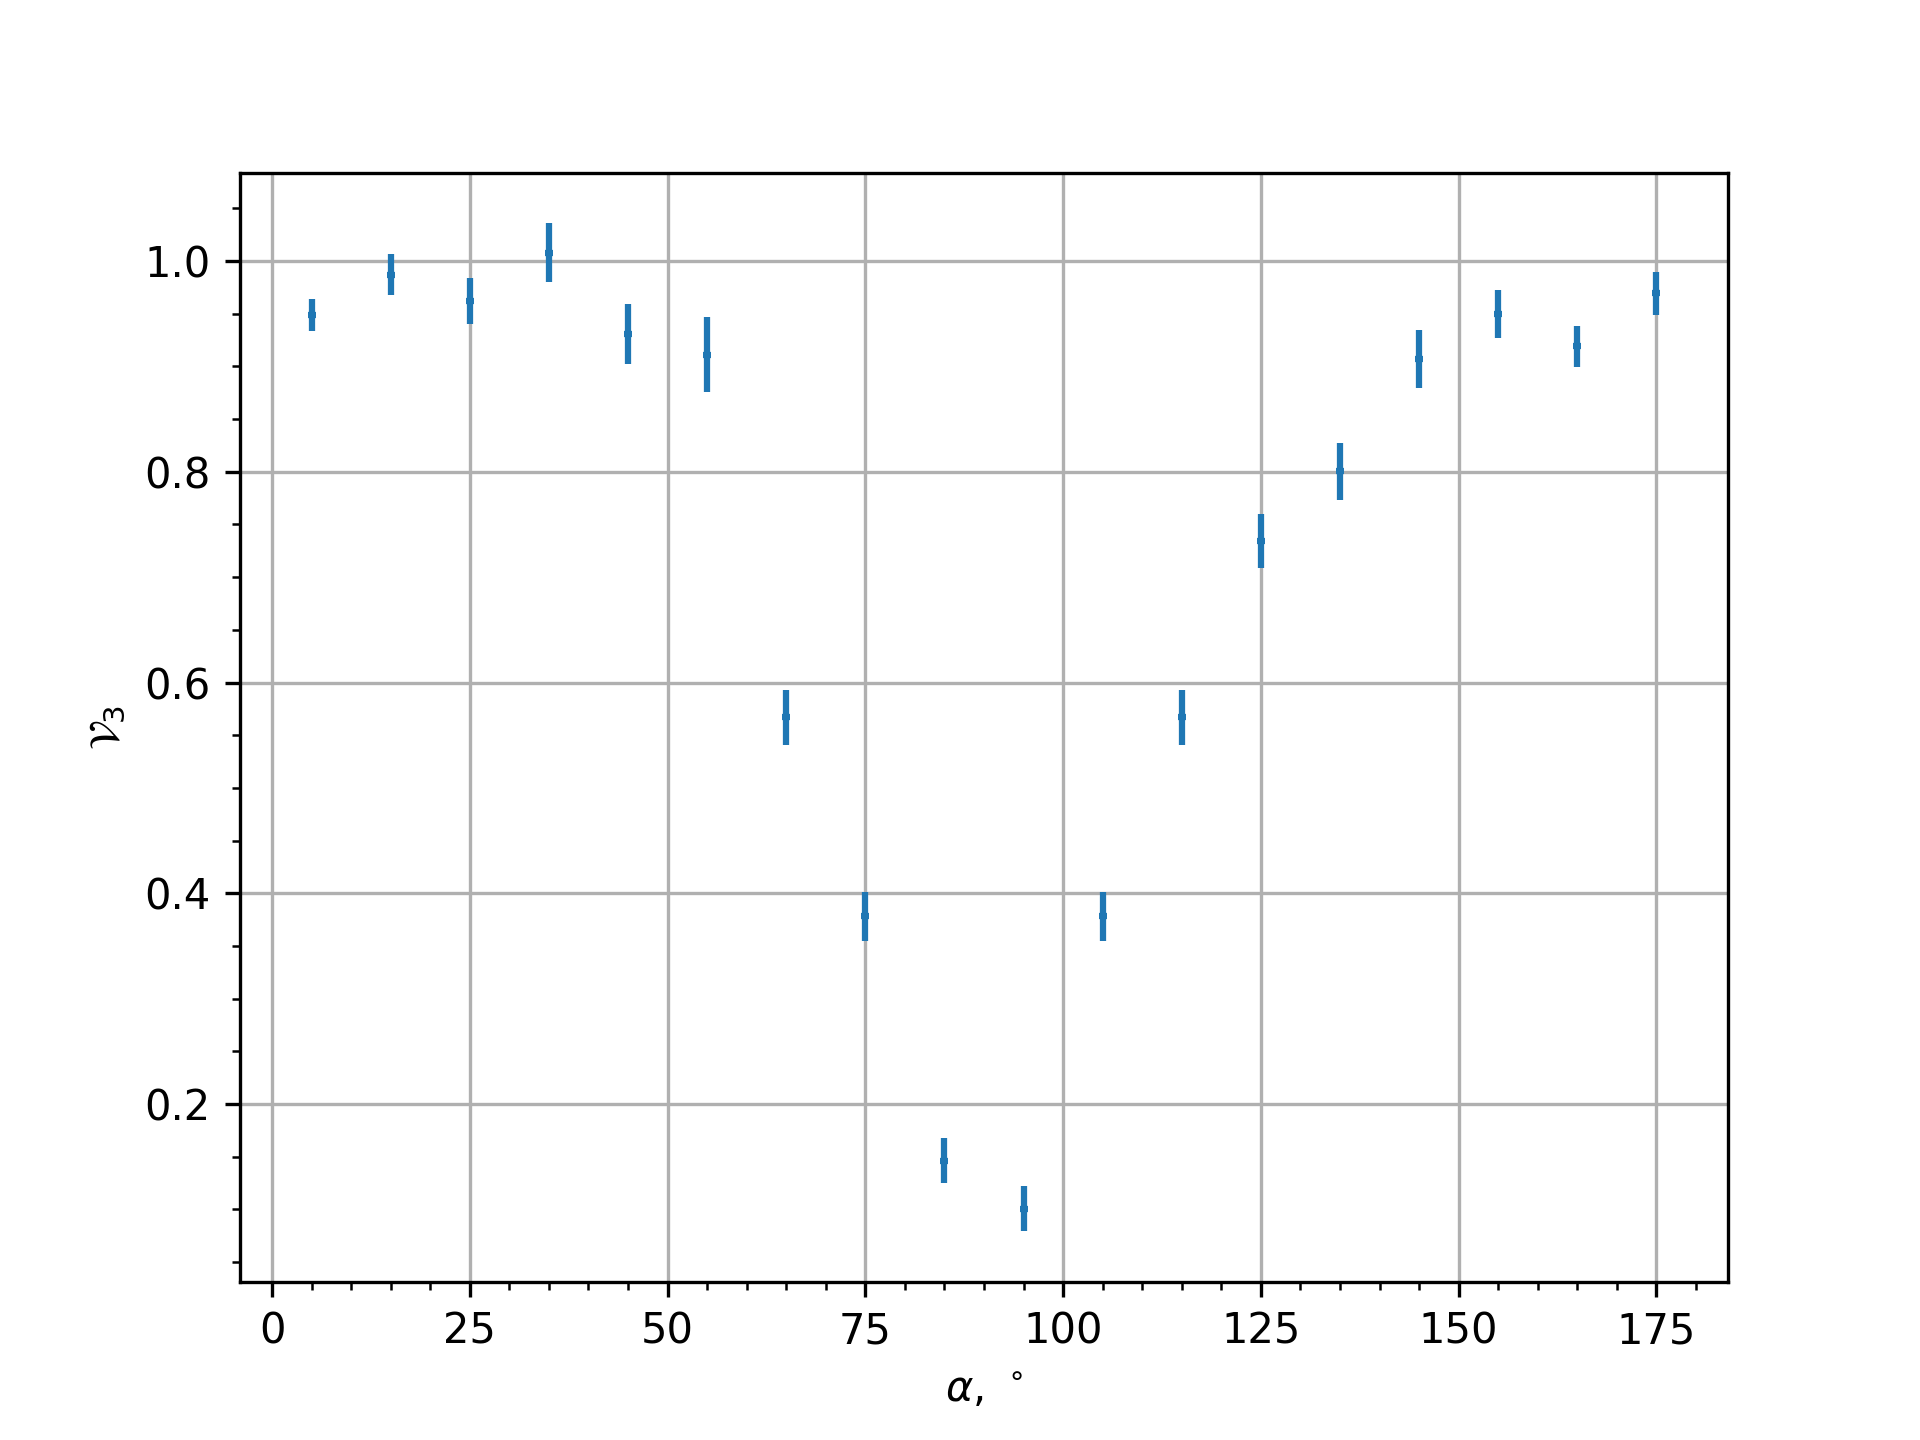
\includegraphics[width=0.9\linewidth]{pic/V(a)}
        \caption{График зависимости видности от угла поворота поляроида П1}
        \label{fig:fig3}
    \end{figure}
    \begin{figure}[b]
        \centering
        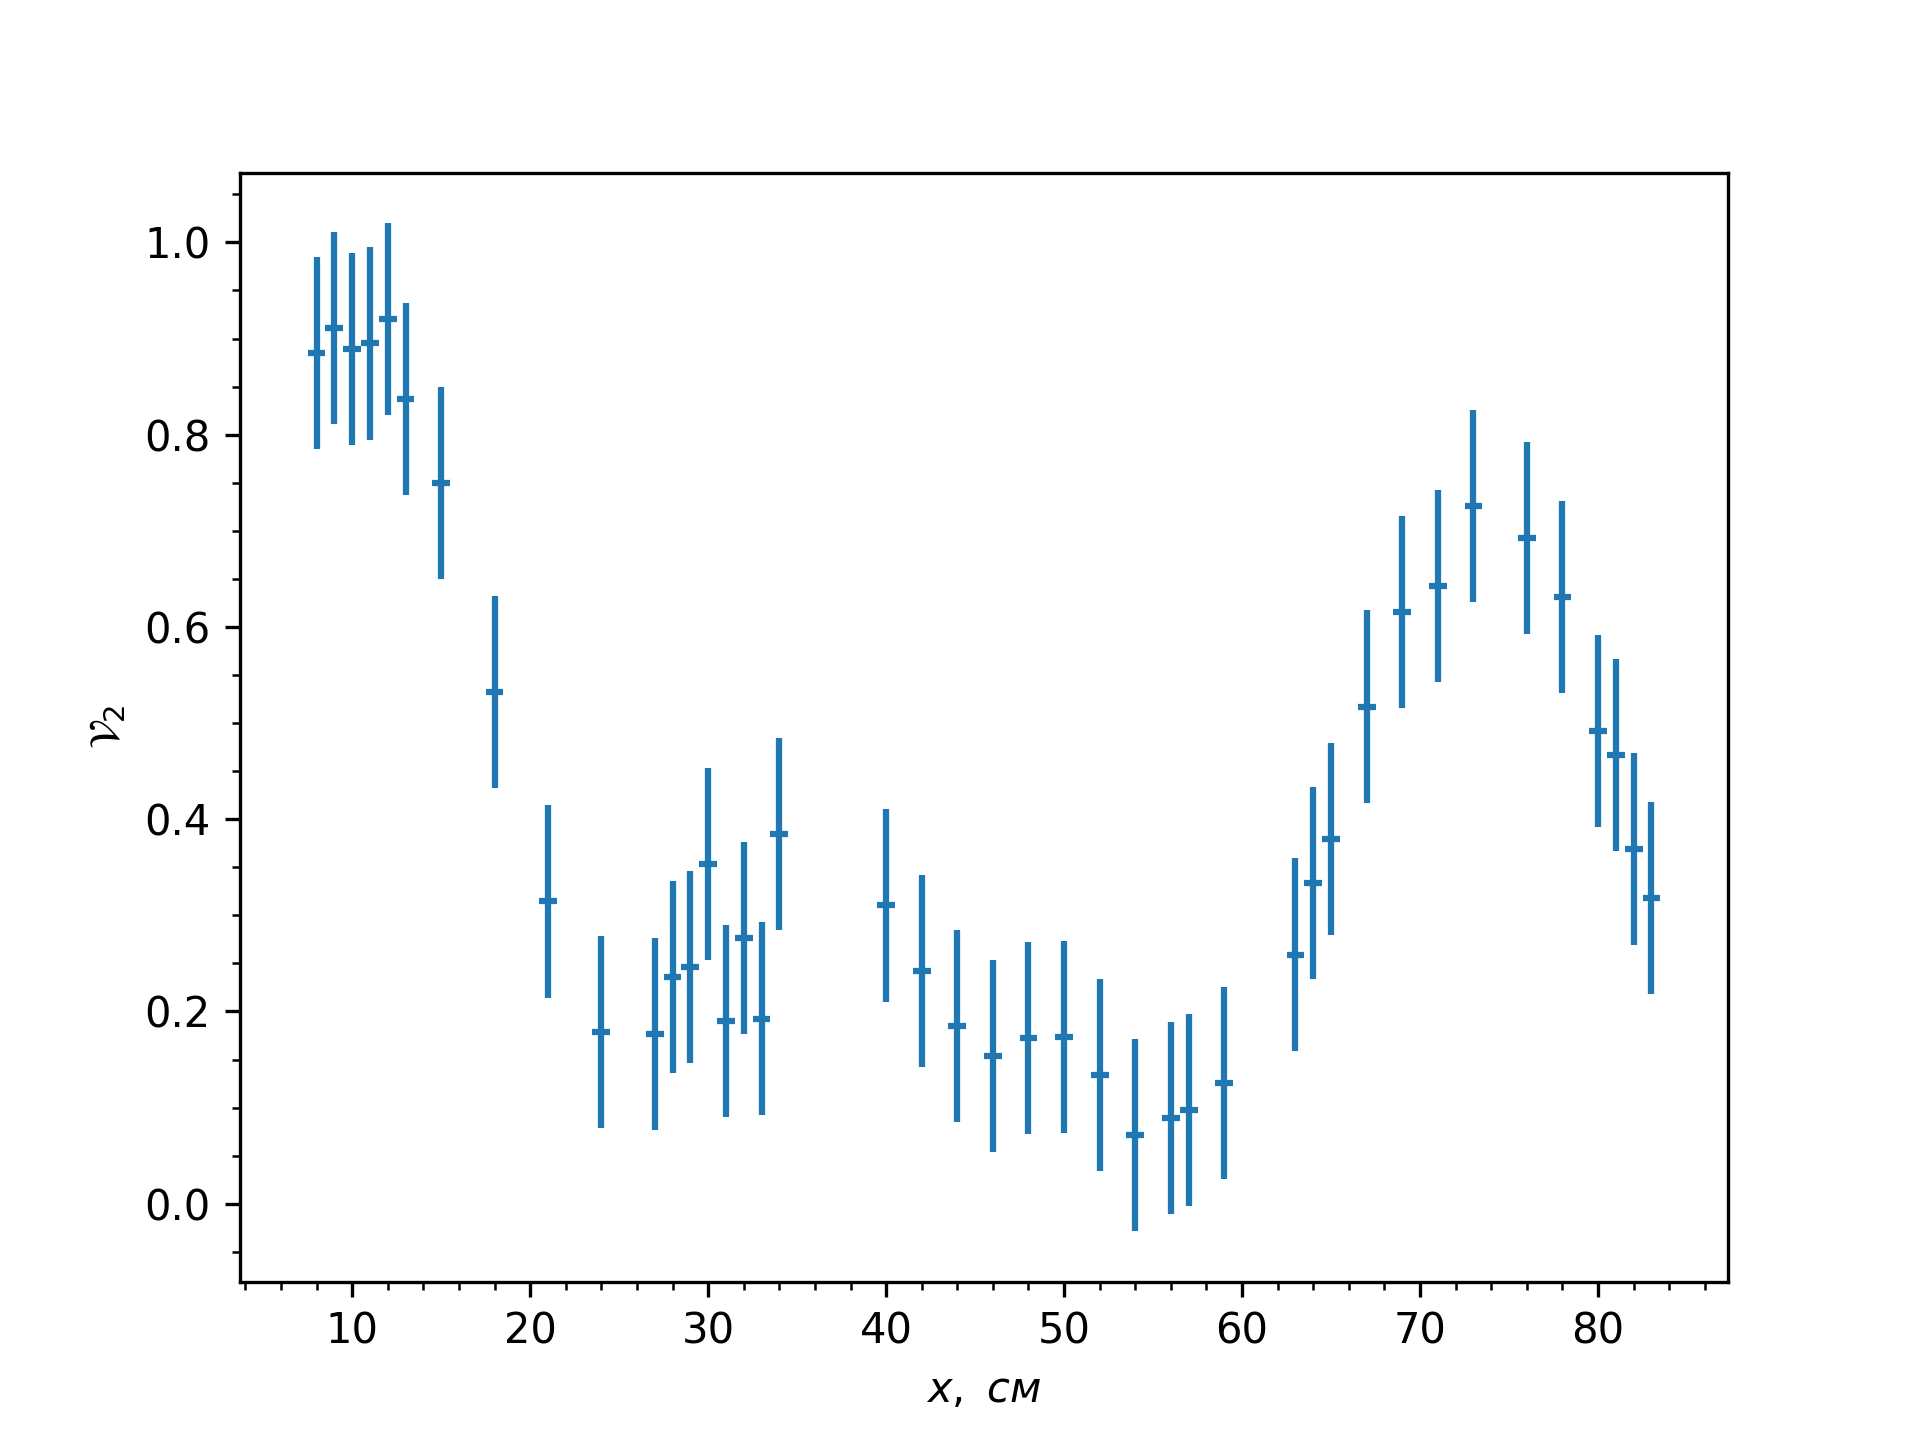
\includegraphics[width=0.9\linewidth]{pic/V(x)}
        \caption{График зависимости видности от координаты блока Б2}
        \label{fig:fig4}
    \end{figure}


    \subsection*{Выводы}
    \begin{itemize}
        \item Зависимость видности от угла поворота поляроида похожа на $\cos^2$ (см рис.\ \ref{fig:fig3}),
        то есть свет поляризован линейно, но направление поляризации изменяется от $0$ до $\pi$
        \item Получена оценка для расстояния между зеркалами (рис.\ \ref{fig:fig4}):
        \[L \approx (32 \pm 2)\ \text{см}\]
        и межмодового расстояния
        \[\Delta \nu \approx (4.0\pm0.3)\cdot10^8\ \text{Гц}\]
    \end{itemize}
\end{document}